\section{\secState{R}Movement Automaton}\label{s:movementAutomatonTheory}

\paragraph{Idea:} The key idea is to create \emph{interface} between \emph{controlled plant} (UAV) and \emph{Avoidance Algorithm} to ensure \emph{Concept Reusability} at maximum degree.  The concept is following:

\begin{enumerate}

    \item \emph{Interface consumes} discrete command chain and guides UAS along \emph{desired trajectory}.
    
    \item \emph{Interface} can be used to \emph{predict trajectory} based on \emph{initial state} and future command chaining. 
\end{enumerate}

Frazolli provided the concept of \emph{Movement Automaton} (def. \ref{def:movementAutomaton}) a specialized type of \emph{Hybrid Automaton} (eq. \ref{eq:hybridAutomaton}), the concept is taken from his works \cite{frazzoli2001robust,frazzoli2000trajectory}. Other aspects and similarities are discussed over this chapter. 


\paragraph{Architecture:} The Movement Automaton can be seen as a consistent hierarchical abstraction of the continuous dynamics, in the sense outlined in \cite{pappas2000hierarchically}: \emph{Any sequence of movement primitives generated by the Movement Automaton results by construction in a trajectory which is executable by the full continuous system. We will give a deeper meaning to hierarchical consistency}. The implementation of our movement automaton is given in (fig.\ref{fig:avoidanceConcept}). 

\paragraph{Optimal Path Generation:} If the maneuvers are instantaneous (i.e. the UAS can transition instantaneously between two different trim trajectories), Reduction of stronger results obtained by Dubins \cite{dubins1957curves} and Reeds \cite{reeds1990optimal} concerning optimal paths for kinematic cars on the plane (see also \cite{soueres1998optimal}). 

\paragraph{Controllability:} The systems controlled by Movement Automaton (as in \cite{lavalle1998rapidly}), is controllable according to our definition, even though it is not
small-time controllable \cite{sussmann1983lie}.

\paragraph{Other Properties:} The other properties of movement automaton, like \emph{Stability, Robustness} and other important control properties are proven in \cite{frazzoli2001robust}.



\paragraph{Example:} The \emph{example} is given in (fig. \ref{fig:movementAutomatonExampleTheory}). The \emph{States} (Barrels) are connected by \emph{Transitions} (green arrows).

\emph{Hover} is neutral and \emph{initial} state, in this place the UAS stays on place and maintains altitude.

\emph{Forward flight} is when \emph{UAS} is flying in frontal direction with constant speed. The speed-up and slow-down is incorporated in \emph{Transition} between \emph{Hover} and \emph{Forward flight} states and its takes some time to execute. \emph{Transitions} between Turning states and \emph{Flight forward} state are almost instant. 

\emph{Steady turn left/right} is when \emph{UAS} is flying in frontal direction and starts steady turning left or right. 

\begin{note}
UAS in (fig. \ref{fig:movementAutomatonExampleTheory}) ignores the vertical maneuvering and it is expected to fly on horizontal plane.
\end{note}


\begin{figure}[H]
    \centering
    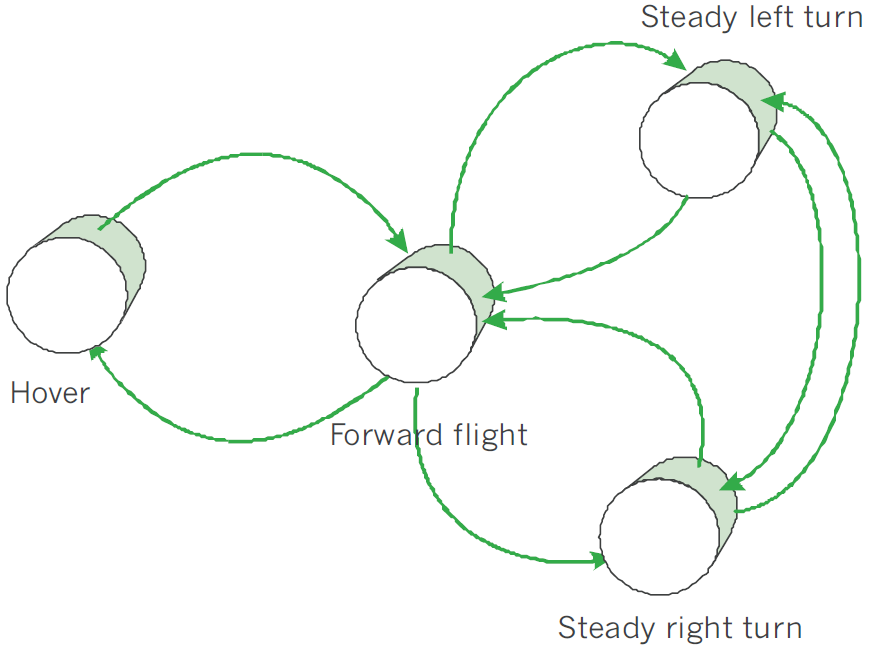
\includegraphics[width=0.55\linewidth]{\FIGDIR/TE030MovementAutomatonFrazzCite} 
    \caption{Movement Automaton for Copter UAS \cite{frazzoli2001robust}.}
    \label{fig:movementAutomatonExampleTheory}
\end{figure}

\paragraph{Used concepts:} The movement automaton is essential part of this work. Supporting the idea, that \emph{Obstacle avoidance framework} can be platform independent. 

The \emph{Movement Automaton} is used as is (sec. \ref{s:MovementAutomatonDefinitionAndProperties}). The implementation is described in (sec. \ref{s:modelMAImplementation}). The testing configuration was given in (tab. \ref{tab:testMovementOrientations}).


